\documentclass[UTF-8, a4paper, 10pt]{article}

\usepackage{xeCJK}
\usepackage{graphicx}
\graphicspath{{figure/}}
\usepackage[unicode]{hyperref}
\hypersetup{colorlinks=true,linkcolor=black}
\usepackage{cite}
\usepackage{indentfirst}
\usepackage{amsmath}
\numberwithin{equation}{section}
\usepackage{listings}
\usepackage{xcolor}
\usepackage{fontspec}
\usepackage{courier}
\usepackage{tikz-timing}

\lstset{
    basicstyle=\scriptsize\ttfamily,
    numbers=left,                                        % 在左侧显示行号
    keywordstyle=\color[RGB]{40,40,255},                 % 设定关键字颜色
    frame=trbl,
    numberstyle=\scriptsize\color{darkgray},           % 设定行号格式
    commentstyle=\it\color[RGB]{0,96,96},                % 设置代码注释的格式
    stringstyle=\ttfamily\slshape\color[RGB]{128,0,0},   % 设置字符串格式
    showstringspaces=false,                              % 不显示字符串中的空格
    language=python,                                     % 设置语言
}


\linespread{1.0}
\setlength{\parskip}{0.5\baselineskip}

\makeatletter
\let\@afterindentfalse\@afterindenttrue
\@afterindenttrue
\makeatother
\setlength{\parindent}{2em}

\addtolength{\topmargin}{-70pt}
\setlength{\oddsidemargin}{0.63cm}
\setlength{\evensidemargin}{\oddsidemargin}
\setlength{\textwidth}{15.66cm}
\setlength{\textheight}{25.00cm}

\newcommand{\chuhao}{\fontsize{42pt}{\baselineskip}\selectfont}
\newcommand{\xiaochuhao}{\fontsize{36pt}{\baselineskip}\selectfont}
\newcommand{\yihao}{\fontsize{28pt}{\baselineskip}\selectfont}
\newcommand{\erhao}{\fontsize{21pt}{\baselineskip}\selectfont}
\newcommand{\xiaoerhao}{\fontsize{18pt}{\baselineskip}\selectfont}
\newcommand{\sanhao}{\fontsize{15.75pt}{\baselineskip}\selectfont}
\newcommand{\sihao}{\fontsize{14pt}{\baselineskip}\selectfont}
\newcommand{\xiaosihao}{\fontsize{12pt}{\baselineskip}\selectfont}
\newcommand{\wuhao}{\fontsize{10.5pt}{\baselineskip}\selectfont}
\newcommand{\xiaowuhao}{\fontsize{9pt}{\baselineskip}\selectfont}
\newcommand{\liuhao}{\fontsize{7.875pt}{\baselineskip}\selectfont}
\newcommand{\qihao}{\fontsize{5.25pt}{\baselineskip}\selectfont}

\begin{document}

\begin{titlepage}
    \begin{center}
    \phantom{Start!}
	\vspace{2cm}
	
\includegraphics[width=350pt]{HUST.pdf} \\
    \vspace{1cm}
     \center{
       	  \textbf{\yihao 实\quad 验\quad 报\quad 告}\\
       	  \vspace{0.5cm}
          \textbf{\sanhao (2017 / 2018学年\quad 第2学期)}
      }
      \vspace{2.5cm}
      \begin{table}[!hbp]
      \centering
      \renewcommand\arraystretch{1.5}
     	\begin{tabular}{|c|c|}
     		\hline
     		课程名称 & 机器学习导论 \\
     		\hline
     		实验名称 & ~~~~~~Decision Tree~~~~~~ \\
     		\hline
     		实验时间&\multicolumn{1}{c|}{2018年5月20日}\\
     		\hline
     		指导教师 & 王邦 \\
     		\hline
     		\end{tabular}     		
       \end{table}
       \vspace{2cm}
      \begin{table}[htbp]
      \centering
      \renewcommand\arraystretch{1.5}
     	\begin{tabular}{|c|c|c|c|}
     		\hline
            \qquad ~~姓名~~~~~  & \qquad ~~游浩然~~~~~  & \qquad 学号~~~~~ & \qquad U201515429~~~~~ \\
     		\hline
     		\end{tabular}
       \end{table}
       \date{2018年5月20日}
     \end{center}
\end{titlepage}

\section{问题重述}
\begin{itemize}
  \item 对课堂上所讲的西瓜数据集,构造决策树。
  \item 根据用户采集的WiFi信息采用决策树预测用户所在房间。
\end{itemize}

\section{西瓜决策树}
\subsection{Python代码实现}
\begin{lstlisting}[language=python]
# -*- coding: utf-8 -*-
"""
@author : Haoran You

"""
from math import log
import operator
import matplotlib
import matplotlib.pyplot as plt

"""
Moudule - Create decision tress for datasets
:createTree(main)
:bestFeature
:calcShannonEnt
:splitDataset
:majorityCnt
"""
def createTree(dataset, label):
    classlist = [example[-1] for example in dataset]
    # no subtree
    if classlist.count(classlist[0]) == len(classlist):
        return classlist[0]
    # no feature
    if len(dataset[0]) == 1:
        return majorityCnt(classlist)
    # choose best feature
    bestFeat = bestFeature(dataset)
    bestFeatLabel = label[bestFeat]
    myTree = {bestFeatLabel:{}}
    del(label[bestFeat])
    # recursion for each subdataset
    feat_values = [example[bestFeat] for example in dataset]
    uniqueVals = set(feat_values)
    for value in uniqueVals:
        sub_label = label[:]
        myTree[bestFeatLabel][value] = createTree(splitDataset(dataset,bestFeat,value), sub_label)
    return myTree

def bestFeature(dataset):
    num_features = len(dataset[0]) - 1
    baseEntropy = calcShannonEnt(dataset)
    bestInfoGain = 0.0
    bestFeat = 0
    for i in range(0, num_features):
        featList = [example[i] for example in dataset]
        uniqueVals = set(featList)
        newEntropy = 0.0
        for value in uniqueVals:
            sub_dataset = splitDataset(dataset, i, value)
            prob = len(sub_dataset) / float(len(dataset))
            newEntropy += prob * calcShannonEnt(sub_dataset)
        infoGain = baseEntropy - newEntropy
        if infoGain > bestInfoGain:
            bestInfoGain = infoGain
            bestFeat = i
    return bestFeat

def calcShannonEnt(dataset):
    num_samples = len(dataset)
    labelCounts = {}
    for feat_vector in dataset:
        current_label = feat_vector[-1]
        if current_label not in labelCounts.keys():
            labelCounts[current_label] = 0
        labelCounts[current_label] += 1
    shannonEnt = 0.0
    for key in labelCounts:
        prob = float(labelCounts[key]) / num_samples
        shannonEnt -= prob * log(prob, 2)
    return shannonEnt

def splitDataset(dataset, axis, value):
    sub_dataset = []
    for feat_vector in dataset:
        if feat_vector[axis] == value:
            reduce_feat_vector = feat_vector[:axis]
            reduce_feat_vector.extend(feat_vector[axis+1:])
            sub_dataset.append(reduce_feat_vector)
    return sub_dataset

def majorityCnt(classlist):
    classCount = {}
    for vote in classlist:
        if vote not in classCount.keys():
            classCount[vote] = 0
        classCount[vote] += 1
    sortedClassCount = sorted(classCount.items(), key=operator.itemgetter(1), reverse=True)
    return sortedClassCount[0][0]

"""
Module - Plot decision tree constructed before
:createPlot(main)
:plotTree
:plotNode
:plotMidText
:getNumLeaves
:getTreeDepth
"""
decisionNode = dict(boxstyle='sawtooth', fc='0.8')
leafNode = dict(boxstyle='round4', fc='0.8')
arrow_args = dict(arrowstyle='<-')

def createPlot(myTree):
    fig = plt.figure(1, facecolor='white')
    fig.clf()
    axprops = dict(xticks=[], yticks=[])
    createPlot.ax1 = plt.subplot(111, frameon=True)
    plotTree.totalW = float(getNumLeaves(myTree))
    plotTree.totalD = float(getTreeDepth(myTree))
    plotTree.xOff = -0.5/plotTree.totalW
    plotTree.yOff = 1.0
    plotTree(myTree, (0.5, 1.0), '')
    plt.show()

def plotTree(myTree, parentPt, nodeTxt):
    num_leaves = getNumLeaves(myTree)
    depth = getTreeDepth(myTree)
    firstStr = list(myTree.keys())[0]
    cntrPt = (plotTree.xOff + (1.0 + float(num_leaves))/2.0/plotTree.totalW, plotTree.yOff)
    plotMidText(cntrPt, parentPt, nodeTxt)
    plotNode(firstStr, cntrPt, parentPt, decisionNode)
    secondDict = myTree[firstStr]
    plotTree.yOff = plotTree.yOff - 1.0/plotTree.totalD
    for key in secondDict.keys():
        if type(secondDict[key]).__name__ == 'dict':
            plotTree(secondDict[key], cntrPt, str(key))
        else:
            plotTree.xOff = plotTree.xOff + 1.0/plotTree.totalW
            plotNode(secondDict[key], (plotTree.xOff, plotTree.yOff), cntrPt, leafNode)
            plotMidText((plotTree.xOff, plotTree.yOff), cntrPt, str(key))
    plotTree.yOff = plotTree.yOff + 1.0/plotTree.totalD

def plotNode(nodeTxt, centerPt, parentPt, nodeType):
    createPlot.ax1.annotate(nodeTxt, xy=parentPt,  xycoords='axes fraction',
             xytext=centerPt, textcoords='axes fraction',
             va="center", ha="center", bbox=nodeType, arrowprops=arrow_args)

def plotMidText(cntrPt, parentPt, txtString):
    # positon for text
    xMid = (parentPt[0]-cntrPt[0])/2.0 + cntrPt[0]
    yMid = (parentPt[1]-cntrPt[1])/2.0 + cntrPt[1]
    createPlot.ax1.text(xMid, yMid, txtString, va="center", ha="center")

def getNumLeaves(myTree):
    numLeaves = 0
    firstStr = list(myTree.keys())[0]
    secondDict = myTree[firstStr]
    for key in secondDict.keys():
        if type(secondDict[key]).__name__=='dict':
            numLeaves += getNumLeaves(secondDict[key])
        else:   numLeaves +=1
    return numLeaves

def getTreeDepth(myTree):
    maxDepth = 0
    firstStr = list(myTree.keys())[0]
    secondDict = myTree[firstStr]
    for key in secondDict.keys():
        if type(secondDict[key]).__name__=='dict':
            thisDepth = 1 + getTreeDepth(secondDict[key])
        else:   thisDepth = 1
        if thisDepth > maxDepth: maxDepth = thisDepth
    return maxDepth

if __name__ == '__main__':
    # load dataset
    f = open('watermelon.txt', 'r', encoding='utf-8')
    label = f.readline()
    label = label.strip().split('  ')
    dataset = [inst.strip().split('  ') for inst in f.readlines()]
    print('feature ', label)
    print('dataset ', dataset)
    # tree structure
    myTree = createTree(dataset, label)
    print('myTree  ', myTree)
    # draw tree
    from pylab import *
    mpl.rcParams['font.sans-serif'] = ['SimHei']
    createPlot(myTree)
\end{lstlisting}
\subsection{结果图}
\begin{figure}[!h]
\begin{tikzpicture}[edge from parent/.style={draw,-latex},
level distance=2cm,
level 1/.style={sibling distance=6.5cm},
level 2/.style={sibling distance=3cm}]
\tikzstyle{every node}=[rectangle,draw]
\node (Root) {纹理}
child {
    node {触感}
    child {
        node {否}
        edge from parent node[left,draw=none] {硬滑}
    }
    child {
        node {是}
        edge from parent node[left,draw=none] {软贴}
    }
    edge from parent node[left,draw=none] {稍糊}
}
child {
    node {根蒂}
    child {
        node {是}
        edge from parent node[left,draw=none] {蜷缩}
    }
    child{
        node {色泽}
        child{
            node {触感}
            child{
                node {是}
                edge from parent node[left,draw=none] {硬滑}
            }
            child{
                node {否}
                edge from parent node[left,draw=none] {软贴}
            }
            edge from parent node[left,draw=none] {乌黑}
        }
        child{
            node {是}
            edge from parent node[left,draw=none] {青绿}
        }
        edge from parent node[left,draw=none] {稍蜷}
    }
    child {
        node {否}
        edge from parent node[left,draw=none] {硬挺}
    }
    edge from parent node[right,draw=none] {清晰}
}
child{
    node {否}
    edge from parent node[left,draw=none] {模糊}
};
\end{tikzpicture}
\caption{A decision tree for evaluating watermelon.}
\label{fig:tree1}
\end{figure}

\section{房间决策树}
\subsection{Python代码实现}
\begin{lstlisting}[language=python]
# -*- coding: utf-8 -*-
"""
@author : Haoran You

"""
from math import log
import csv
import os
import random
import matplotlib.pyplot as plt
from Task1 import *

def devidetraincsv():
    trainDT = csv.reader(open('TrainDT.csv', 'r'))
    dataset = []
    for line in trainDT:
        dataset.append(line)
    del(dataset[0])
    time_list = list(set([int(example[-1]) for example in dataset]))
    BSSID_list = list(set([example[0] for example in dataset]))
    label_dict = {}
    for item in dataset:
        label_dict[item[-1]] = item[2]
    pre_whole_train = []
    for i in range(0, len(time_list)):
        new_dict = {}
        for j in range(0, len(BSSID_list)):
            new_dict[BSSID_list[j]] = 0
        pre_whole_train.append(new_dict)
    for item in dataset:
        pre_whole_train[int(item[-1])-1][item[0]] = float(item[1])
    whole_train = []
    fin_label = 0
    for item in pre_whole_train:
        fin_label += 1
        new_list = []
        for keys in item.keys():
            new_list.append(item[keys])
        new_list.append(label_dict[str(fin_label)])
        whole_train.append(new_list)
    num_train = int(0.9*len(whole_train))
    num_val = len(whole_train) - num_train
    train = random.sample(whole_train, num_train)
    val = random.sample(whole_train, num_val)
    return train, val, BSSID_list

def dividetestcsv(feature):
    testDT = csv.reader(open('TestDT.csv', 'r'))
    dataset = []
    for line in testDT:
        dataset.append(line)
    del (dataset[0])
    time_list = list(set([int(example[-1]) for example in dataset]))
    BSSID_list = feature
    pre_whole_test = []
    for i in range(0, len(time_list)):
        new_dict = {}
        for j in range(0, len(BSSID_list)):
            new_dict[BSSID_list[j]] = 0
        pre_whole_test.append(new_dict)
    for item in dataset:
        pre_whole_test[int(item[-1]) - 1][item[0]] = float(item[1])
    whole_test = []
    fin_label = 0
    for item in pre_whole_test:
        fin_label += 1
        new_list = []
        for keys in item.keys():
            new_list.append(item[keys])
        whole_test.append(new_list)
    return whole_test

def discretization(dataset):
    for i in range(0, len(dataset[0])-1):
        rss_list = [example[i] for example in dataset]
        num = len(rss_list)
        for k in range(0, num):
            if rss_list[k] == 0.0:
                dataset[k][i] = 0
            else:
                dataset[k][i] = 1
    return dataset

def predict_val(dataset, feature, tree):
    label = [example[-1] for example in dataset]
    i = 0
    total_num = len(label)
    corr_num = 0
    for item in dataset:
        for keys in tree.keys():
            index = feature.index(keys)
            sub_tree = tree[keys][item[index]]
            if isinstance(sub_tree, dict):
                pred = find_leaf(item, feature, sub_tree)
            else:
                pred = sub_tree
        if pred == label[i]:
            corr_num += 1
        i += 1
    acc = corr_num / total_num
    return acc

def predict(dataset, feature, tree):
    if os.path.exists('results.csv'):
        os.remove('results.csv')
    f = open('results.csv', 'a', newline='')
    csv_write = csv.writer(f, dialect='excel')
    i = 1
    for item in dataset:
        for keys in tree.keys():
            index = feature.index(keys)
            sub_tree = tree[keys][item[index]]
            if isinstance(sub_tree, dict):
                pred = find_leaf(item, feature, sub_tree)
            else:
                pred = sub_tree
        i += 1
        result = []
        result.append(i)
        result.append(pred)
        csv_write.writerow(result)

def find_leaf(item, feature, tree):
    for keys in tree.keys():
        index = feature.index(keys)
        sub_tree = tree[keys][item[index]]
        if isinstance(sub_tree, dict):
            pred = find_leaf(item, feature, sub_tree)
        else:
            pred = sub_tree
    return pred

if __name__ == '__main__':
    train_dataset, val_dataset, feature = devidetraincsv()
    test_dataset = dividetestcsv(feature)
    print('feature   ', feature)
    print('num_train ', len(train_dataset))
    print('num_val   ', len(val_dataset))
    train_dataset = discretization(train_dataset)
    myTree = createTree(train_dataset, feature.copy())
    print(myTree)
    createPlot(myTree)
    val_dataset = discretization(val_dataset)
    acc = predict_val(val_dataset, feature.copy(), myTree)
    print('accuracy  ', acc)
    test_dataset = discretization(test_dataset)
    predict(test_dataset, feature.copy(), myTree)
\end{lstlisting}

\subsection{结果图}
\begin{figure}[!h]
\begin{tikzpicture}[edge from parent/.style={draw,-latex},
level distance=1.5cm,
level 1/.style={sibling distance=8cm},
level 2/.style={sibling distance=3cm}]
\tikzstyle{every node}=[rectangle,draw]
\node (Root) {06:69:6c:0a:bf:02}
child {
    node {4a:ee:65:e1:e1:85}
    child {
        node {8c:a6:df:91:51:45}
        child{
            node {2}
            edge from parent node[left,draw=none] {0}
        }
        child{
            node {4}
            edge from parent node[left,draw=none] {1}
        }
        edge from parent node[left,draw=none] {0}
    }
    child {
        node {4}
        edge from parent node[left,draw=none] {1}
    }
    edge from parent node[left,draw=none] {0}
}
child {
    node {24:05:0f:9b:e7:63}
    child{
        node {06:69:6c:0a:be:fa}
        child{
            node {d4:ee:07:50:f1:3c}
            child{
                node {06:69:6c:0a:bf:06}
                child{
                    node{4a:ee:65:e1:e1:85}
                    child{
                        node{3}
                        edge from parent node[left,draw=none] {0}
                    }
                    child{
                        node{4}
                        edge from parent node[left,draw=none] {1}
                    }
                    edge from parent node[left,draw=none] {0}
                }
                child{
                    node{1}
                    edge from parent node[left,draw=none] {1}
                }
                edge from parent node[left,draw=none] {0}
            }
            child{
                node {2}
                edge from parent node[left,draw=none] {1}
            }
            edge from parent node[left,draw=none] {0}
        }
        child{
            node {3}
            edge from parent node[left,draw=none] {1}
        }
        edge from parent node[left,draw=none] {0}
    }
    child {
        node {1}
        edge from parent node[left,draw=none] {1}
    }
    edge from parent node[right,draw=none] {1}
};
\end{tikzpicture}
\caption{A decision tree for evaluating roomlabel. 0 presents no signal received, 1 means inversely.}
\label{fig:tree1}
\end{figure}

\end{document} 